% Options for packages loaded elsewhere
\PassOptionsToPackage{unicode}{hyperref}
\PassOptionsToPackage{hyphens}{url}
%
\documentclass[
  man,floatsintext,
  man]{apa6}

\usepackage{amsmath}
\usepackage{amsthm}
\usepackage{framed}
\usepackage{pifont}
\usepackage{listings}
\usepackage{tikz}
\usepackage{hyperref}
\usepackage{float}
\usepackage{paralist}
\usepackage{xcolor}
\usepackage{tikz}
\usepackage{siunitx}
\usepackage{float}
\newenvironment{smalltable}{\begin{table}[H]\footnotesize}{\end{table}}
\ifLuaTeX
  \usepackage{selnolig}  % disable illegal ligatures
\fi
\usepackage[]{biblatex}
\addbibresource{r-references.bib}
\IfFileExists{bookmark.sty}{\usepackage{bookmark}}{\usepackage{hyperref}}
\IfFileExists{xurl.sty}{\usepackage{xurl}}{} % add URL line breaks if available
\urlstyle{same}
\hypersetup{
  pdftitle={Discover the Influence of Econmic Variables on CPI},
  pdfauthor={Ruiming Min1, Zicheng Wang2, Qi Yang3, \& Shumeng Zhang4},
  pdflang={en-EN},
  hidelinks,
  pdfcreator={LaTeX via pandoc}}

\title{Discover the Influence of Econmic Variables on CPI}
\author{Ruiming Min\textsuperscript{1}, Zicheng Wang\textsuperscript{2}, Qi Yang\textsuperscript{3}, \& Shumeng Zhang\textsuperscript{4}}
\date{}


\shorttitle{CPI and the Economic Variables}

\authornote{

Enter author note here.

The authors made the following contributions. Ruiming Min: Conceptualization, Data curation, Resources, Formal Analysis, Methodology, Writing - Original Draft Preparation, Writing - Review \& Editing; Zicheng Wang: role 3, role 4; Qi Yang: role 1, role 2; Shumeng Zhang: role 3, role 4.

}

\affiliation{\vspace{0.5cm}\textsuperscript{2} UIUC}

\abstract{%
One or two sentences providing a \textbf{basic introduction} to the the problem being addressed by this study.
One sentence summarizing the main result.
Two or three sentences explaining what the \textbf{main result} reveals in direct comparison to what was thought to be the case previously, or how the main result adds to previous knowledge.
One or two sentences to put the results into a more \textbf{general context}.
Two or three sentences to provide a \textbf{broader perspective}, readily comprehensible to a scientist in any discipline.
}



\begin{document}
\maketitle

\hypertarget{introduction}{%
\section{Introduction}\label{introduction}}

Economics is a highly applicable field for utilization of time series analysis. The volume of data is abundant and inherently index with time. By using the time series statistical models, we can leverage historical data and catch trends and patterns for the data and make reasonable predictions.

\hypertarget{consumer-price-index-cpi}{%
\subsection{Consumer Price Index (CPI)}\label{consumer-price-index-cpi}}

In this project, we are analyzing the Consumer Price Index (CPI), a widely-used economic indicator that measures changes in the average price level of a basket of goods in an economic entity. It is commonly used to track inflation and assess price changes. A positive CPI value indicates inflation, while a negative value indicates deflation in the market. The goods' prices selected to calculate this index typically represent the overall prices of goods and services in society.
CPI is calculated relative to the price in the previous time period, which is assigned a value of 100. The percentage difference between the current price and the previous price is reflected in the index using a weighted average formula. Generally, a CPI increase of 3\% is considered inflation, while values over 5\% may indicate significant inflation in the economic entity. There are also some variants of CPI. Such as core CPI which excludes volatile food and energy prices, and regional CPIs, which focus on CPI values in specific geographical areas.
Given the critical role CPI plays in the economic landscape, we will introduce our approach to explore temporal and seasonal data patterns of CPI.

\hypertarget{related-research}{%
\subsection{Related Research}\label{related-research}}

One of the seminal paper in this field is by James H. Stock\autocite{STOCK1999293}. His research primarily centers around Phillips curve, which describes the connection of inflation and unemployment rate. In our own research, employment stands out as a crucial metrics that we analyze.
In recent years, there are some researches \autocite{NGUYEN2023e20730} \autocite{BARKAN20231145} employing machine learning and deep neural network for the prediction. These models exists strong performance, particularly with large dataset and when forecasting extended timeframes. However, it is important to note that due to the nature of these complex machine learning models, they often lack interpretability or the ability to provide clear explanations for their predictions.

\hypertarget{data-sources-and-analysis-approach}{%
\subsection{Data Sources and Analysis Approach}\label{data-sources-and-analysis-approach}}

Our primary data sources includes critical economic indicators, including the unemployment rate, government expenditure, investment, and consumption. These indicators play a pivotal role in measuring the level of economic activity within the entity. Furthermore, in our analytical approach, we use lagged and transformed Consumer Purchasing Index values, in conjunction with time-related variables, to enrich the comprehensiveness and precision of our assessments. It's worth noting that all these data elements are aligned with our response variable and are collected on a monthly basis.

\hypertarget{methods}{%
\section{Methods}\label{methods}}

To address the problem at hand, we used the following three steps to analyze the data: 1. detrending, 2. lag analysis, 3. adding the economic variables.

\hypertarget{detrending}{%
\subsection{Detrending}\label{detrending}}

Observating the original data, the CPI has a significantly exponential trend. So we first use a exponential model to fit the data.
Moreover, according to the nature of the CPI, which is highly related to inflation rate, and the avarage of inflation rate, we choose 1.05 as the base of the exponential model.

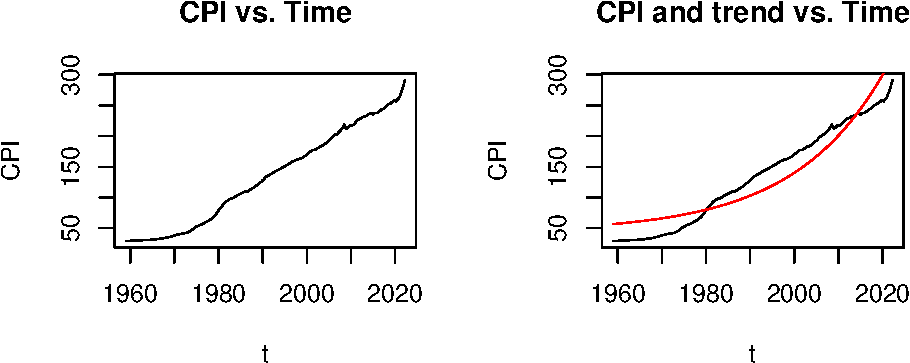
\includegraphics{stat429_group2_final_proj_files/figure-latex/unnamed-chunk-1-1.pdf}

\hypertarget{adding-the-economic-variables}{%
\subsection{Adding the economic variables}\label{adding-the-economic-variables}}

After the detrending and adding the first order lag of CPI, the time series of CPI, \(\{CPI(t)\}\), has became \(CPI(t) = T(t) + CPI(t-1) + Y_t\).

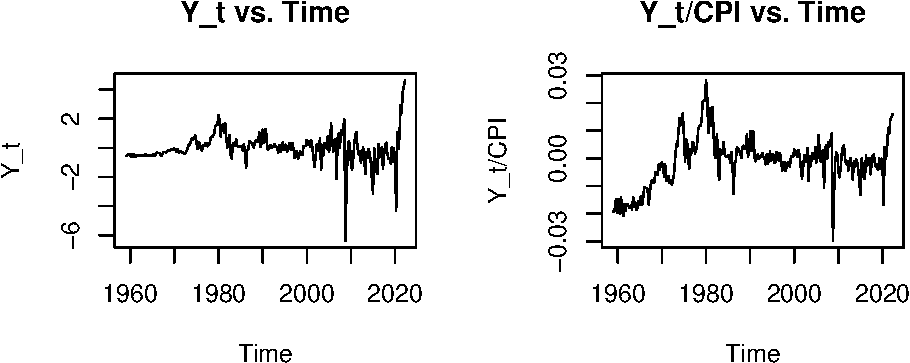
\includegraphics{stat429_group2_final_proj_files/figure-latex/unnamed-chunk-2-1.pdf}

The plot above shows that \(Y_t\) still dose not behave like a white noise.
Additionally, the significant depressions at 2008 and 2020 and the significant peak at 1979 reflexed the influence of the economic crisis\autocite{gross2019iran} \autocite{williams2010uncontrolled} \autocite{forbes_2019_strange_new_world}.
So we add some economic variables to the model to regress the final model.
Also, we add the sine functions of time to the model to fit the seasonal effect of the business cycle.

According to the nature of CPI \autocite{blanchard2004macroeconomics}, \(CPI(t) = \frac{\sum_{i \in \mathcal{P}} P_{i,t} Q_i}{\sum_{i \in \mathcal{P}} P_{i,0} Q_i}\), where \(\mathcal{P}\) is the set of all goods and services, \(P_{i,t}\) is the price of good or service \(i\) at time \(t\), and \(Q_i\) is the quantity of good or service \(i\) at the base period.
Since the Wage-Setting Relation, \(W = \mathcal{A} P^e F(u,z)\), where \(W\) is the nominal wage, \(\mathcal{A}\) is the price mark-up, \(F(u,z)\) is the function of unemployment rate and other variables, \(u\) is the unemployment rate, and z is the output(GDP), and the Price-Setting Relation, \(P = (1+m)\frac{W}{\mathcal{A}}\), where \(m\) is the desired mark-up,
it is concluded as
\[CPI(t) = \frac{\sum_{i \in \mathcal{P}} (1+m_i) \frac{W_i}{\mathcal{A}} Q_i}{\sum_{i \in \mathcal{P}} P_{i,0} Q_i} = \frac{\sum_{i \in \mathcal{P}} (1+m_i) P_{i,t}^e F(u,z) Q_i}{\sum_{i \in \mathcal{P}} P_{i,0} Q_i}\].

To simplify the formular, we assume \(m_i = m \,\, \forall i\) and \(P_{i,t}^e = P_{i,t-1}\), we get \(CPI(t) = CPI(t-1) (1+m) F(u,z)\).
By the assumption of \(m\) is small and \(F(u,z) = 1 - \alpha u + \beta z\), we get \(CPI(t) = CPI(t-1) (1+m) (1 - \alpha u + \beta z)\) \(\cong CPI(t-1) ( 1 + m - \alpha u - \beta z)\).
We could conclude \(CPI(t)=CPI(t-1)(1 + m - \alpha u + \beta z)\).
For easy-computation, we assume CPI(t-1) is a constent we get \(CPI(t)=CPI_0(1 + m - \alpha u + \beta z)\).
Therefore we add the unemployment rate, the real consumption, real grovement spending, and the real investment to the model.

Moreover, we add the sine functions of time to the model to fit the seasonal effect of the business cycle and the square of time to fit the trend of the CPI.

To summarize the first model, we get the model as follows:

\begin{align*}
CPI(t) =& a_0 + a_1 \cdot 1.05^t  + a_2 (t-1959)^2 && (\text{trend})\\
& + a_3 \sin\left(\frac{2\pi(t-1959)}{40}\right) + a_4 \sin\left(\frac{2\pi(t-1980)}{24}\right) + a_5 \sin\left(\frac{2\pi(t-1980)}{48}\right) && (\text{business cycle})\\
& + b_1 C_t + b_2 u_t + b_3 G_t + b_4 I_t + W_t && (\text{economic variables})
\end{align*}

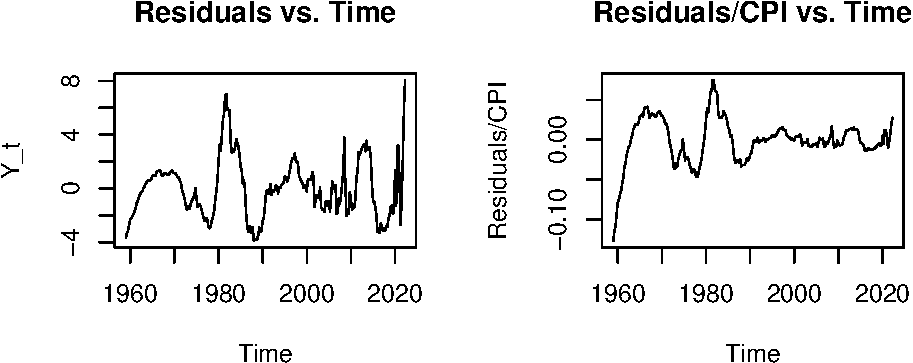
\includegraphics{stat429_group2_final_proj_files/figure-latex/unnamed-chunk-3-1.pdf}

The plot above shows that residuals still dose not behave like a white noise.
Therefore, we will use ACf to figure out weather or not the data has lags and improve our model.

\hypertarget{lag-analysis}{%
\subsection{Lag Analysis}\label{lag-analysis}}

After conclude the first model, we use PACF to figure out weather or not the data has lags.
From the plot below, the data has one lags.
Therefore, the CPI may be a AR(1) process
and we improve our model by adding the first oreder lag of CPI to the model.

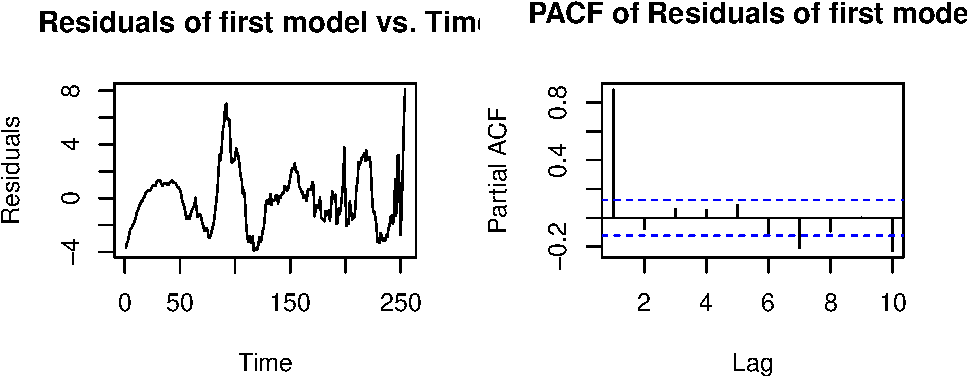
\includegraphics{stat429_group2_final_proj_files/figure-latex/unnamed-chunk-4-1.pdf}

Moreover, we delete the square of time from the model since it is not significant.

To summarize the second model, we get the final model as follows:

\begin{align*}
CPI(t) =& a_0 + a_1 \cdot 1.05^t + a_2 CPI(t-1)  && (\text{trend and lags})\\
& + a_3 \sin\left(\frac{2\pi(t-1959)}{40}\right) + a_4 \sin\left(\frac{2\pi(t-1980)}{24}\right) + a_5 \sin\left(\frac{2\pi(t-1980)}{48}\right) && (\text{business cycle})\\
& + b_1 C_t + b_2 u_t + b_3 G_t + b_4 I_t + W_t && (\text{economic variables})
\end{align*}

where \(W_t\) is a white noise.

\hypertarget{results}{%
\section{Results}\label{results}}

\hypertarget{fitting-results}{%
\subsection{Fitting Results}\label{fitting-results}}

The fitted result of the model is shown below. The plot shows that the model fits the data well.

\bgroup \begin{table}[H]\footnotesize
    \centering
    \begin{tabular}{
      l
      S
      S[table-format=3.4]
      S[table-format=2.3]
      S[table-format=1.4e-2]
    }
    \toprule
    {Coefficients} & {Estimate} & {Std. Error} & {t value} & {Pr(>|t|)}  \\
    \midrule
(Intercept) & 2.159e+00 & 4.662e-01 & 4.632 & 5.90e-06  \\
I(1.05\textasciicircum t) & -8.779e-42 & 1.245e-42 & -7.050 & 1.83e-11\\
sin\_1 & -3.881e+00 & 6.540e-01 & -5.934 & 1.01e-08\\
sin\_2 & -1.028e+00 & 1.593e-01 & -6.455 & 5.80e-10 \\
sin\_3 & -3.760e+00 & 9.484e-01 & -3.965 & 9.66e-05  \\
CPI\_lag1 & 9.735e-01 & 1.351e-02 & 72.033 & < 2e-16  \\
unemp\_rate & 1.847e-01 & 5.406e-02 & 3.416 & 0.000745  \\
grove\_exp & 6.250e-04 & 2.178e-04 & 2.870 & 0.004470  \\
invest & 7.797e-04 & 3.737e-04 & 2.087 & 0.037966  \\
consump\_real & 3.423e-03 & 3.337e-04 & 10.259 & < 2e-16 \\
    \bottomrule
\end{tabular}
\end{table}\egroup

\[
\begin{aligned}
&\text{Residual standard error: 0.8011 on 244 degrees of freedom} \\
&\text{Multiple R-squared: 0.9999, Adjusted R-squared: 0.9999} \\
&\text{F-statistic: 2.688e+05 on 9 and 244 DF, p-value: < 2.2e-16}
\end{aligned}
\]

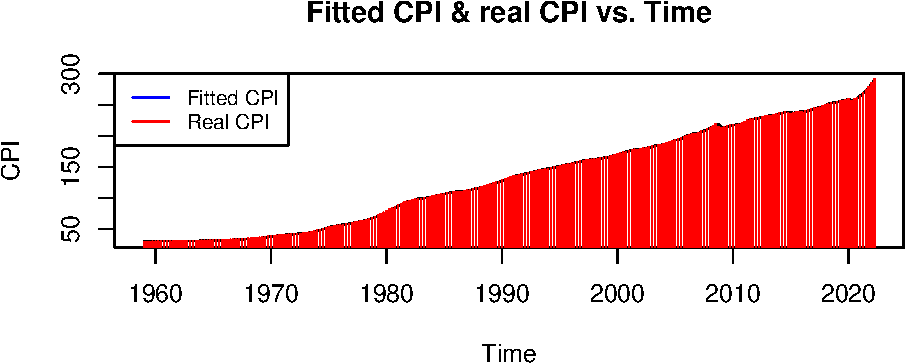
\includegraphics{stat429_group2_final_proj_files/figure-latex/unnamed-chunk-5-1.pdf}

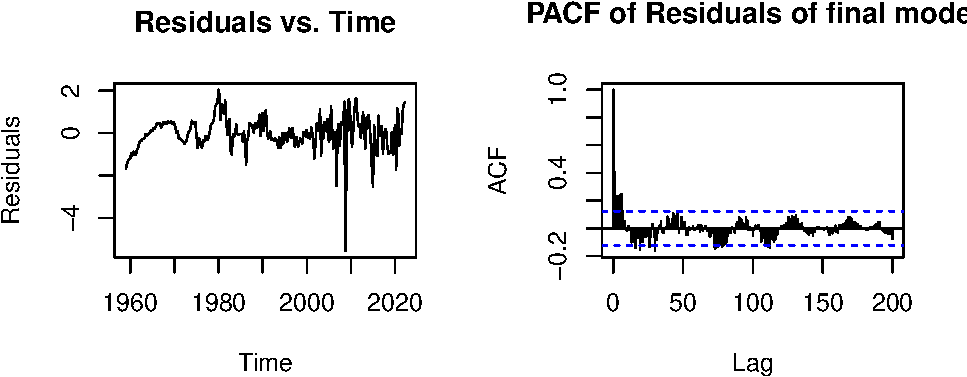
\includegraphics{stat429_group2_final_proj_files/figure-latex/unnamed-chunk-6-1.pdf}

We can find althought there are still a depression at 2010 but the residuals of the final model seem like a white noise at other point.
And the ACF plot shows that most of thecorrelation of residuals are with in the confident interval.

\hypertarget{forecasting-results}{%
\subsection{Forecasting Results}\label{forecasting-results}}

The forecasting result of the model is shown below. The plot shows that the model fits the data well.

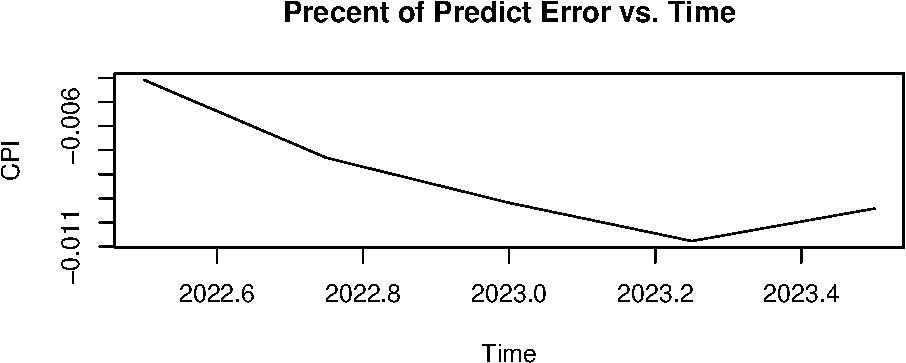
\includegraphics{stat429_group2_final_proj_files/figure-latex/unnamed-chunk-7-1.pdf}

And the mean square error of the model is 7.185918e-05

\hypertarget{rest}{%
\subsubsection{rest}\label{rest}}

A presentation of the results of your analysis. Interpretations should include a discussion of statistical versus practical import of the results.

\hypertarget{discussion}{%
\section{Discussion}\label{discussion}}

A synopsis of your findings and any limitations your study may suffer from.

\newpage

\hypertarget{references}{%
\section{References}\label{references}}

\hypertarget{appendix-optional}{%
\section{Appendix (Optional)}\label{appendix-optional}}

Any R codes or less important R outputs that you wanted to keep- can go in here.


\printbibliography

\end{document}
